%%%%%%%%%%%%%%%%%%%%%%%%%%%%%%%%%%%%%%%%%

%%%%%%%%%%%%%%%%%%%%%%%%%%%%%%%%%%%%%%%%%

%----------------------------------------------------------------------------------------
%	PACKAGES AND DOCUMENT CONFIGURATIONS
%----------------------------------------------------------------------------------------

\documentclass{article}
\usepackage{siunitx} % Provides the \SI{}{} command for typesetting SI units
\usepackage{graphicx} % Required for the inclusion of images
\usepackage[square, numbers, comma, sort&compress]{natbib}
\usepackage[small, bf]{caption} 
\usepackage{booktabs} % Horizontal rules in tables
\usepackage[section]{placeins}
\usepackage{amsmath}
\captionsetup[table]{skip=10pt}
\setlength\parindent{0pt} % Removes all indentation from paragraphs


%----------------------------------------------------------------------------------------
%	DOCUMENT INFORMATION
%----------------------------------------------------------------------------------------
\title{Determining the ground-state energy of the hydrogen molecule with variational Monte Carlo (VMC)} % Title

\author{Bas \textsc{Nijholt}} % Author name

\date{\today} % Date for the report

\begin{document}

\maketitle % Insert the title, author and date

\begin{center}
\begin{tabular}{l r}
Date started: & March 6, 2014 \\ 
Instructor: & Dr. J.M. Thijssen
\end{tabular}
\end{center}

% If you wish to include an abstract, uncomment the lines below
\begin{abstract}
The potential-energy curve for the electronic ground state of the hydrogen molecule has been calculated using the variational quantum Monte Carlo (VMC) method of solving the Schr\"odinger equation in the Born-Oppenheimer approximation. The trail wavefunction sampling was carried out in a 6-dimensional configuration space and contained the simple form of two Hartree-Fock single electron orbitals multiplied by a Jastow-factor. The validity of the VMC method was checked by first applying it to the quantum harmonic oscillator. For H$_2$ we found the dissociation energy $D_e = 36 219(70)$ cm$^{-1}$, the equilibrium internuclear distance $s=1.405$ $a_0$ with a ground-state energy of $-1.151093(14)$ Ha which is in good agreement to experimental data.
\end{abstract}

%----------------------------------------------------------------------------------------
%	SECTION 1
%----------------------------------------------------------------------------------------

\section{Introduction}
The determination of energies for molecular systems is a problem of general interest in chemistry and physics. We report here calculations of the ground state energy for the simplest molecular system containing a electron pair bond using the Variational Monte Carlo (VMC) method using the Born-Oppenheimer approximation. Accurate potential energy curves as functions of the inter-atomic distance have been computed for the ground state of the hydrogen molecule. \\

These calculations also provide us with an example of a computationally demanding problem which is well suited for parallel computing.\\ 

There is a long history of increasingly accurate theoretical calculations of the energy of the hydrogen molecule and increasingly accurate experimental measurements of the dissociation energy. The history of accurate calculations of energies for H$_2$ begins with the 1933 work of James and Coolidge \citep{james1933ground} which represented one of the first successes in solving the Schr\"odinger equation for molecules. In the 1960's, more accurate results for the hydrogen molecule were obtained by Kolos and Roothaan \citep{kolos1960accurate} and by Kolos and Wolniewicz \citep{kolos1963nonadiabatic, kol1964accurate, kol1965potential, kolos1968improved} which established the foundation for future calculations. \\

The effectiveness of the VMC method is demonstrated by applying it to a very simple quantum mechanical system, the harmonic oscillator from which we know the exact results.

\section{Variational Monte Carlo}
Variational Monte Carlo (VMC) is based on a direct application of Monte Carlo integration to explicitly correlated many-body wavefunctions. The variational principle of quantum mechanics, derived in the following section, states that the energy of a trial wavefunction will be greater than or equal to the energy of the exact wavefunction\citep{griffiths1995introduction}.

\subsection{Variational principle}
In quantum mechanics, the variational method is one way of finding approximations to the lowest energy eigenstate or ground state, and some excited states. The basis for this method is the variational principle \citep{griffiths1995introduction, sakurai1994modern}. The method consists in choosing a "trial wavefunction" depending on one or more parameters, and finding the values of these parameters for which the expectation value of the energy is the lowest possible. The wavefunction obtained by fixing the parameters to such values is then an approximation to the ground state wavefunction, and the expectation value of the energy in that state is an upper bound to the ground state energy.\\

The variational principle of quantum mechanics may be derived by expanding a normalized trial wavefunction, $\psi_{T}$, in terms of the exact normalized eigenstates of the Hamiltonian

\begin{equation}
 \psi_T=\sum_{i=0}^{\infty} c_{i} \psi_i \;\;\;,
\end{equation}

where the expansion coefficients, $c_{i}$, are normalised 

\begin{equation}
\sum_{i=0}^{\infty} \vert c_{i}\vert^2=1 \;\;\;.
\end{equation}

The expectation of the many-body Hamiltonian, $\hat{H}$, may be evaluated 

\begin{align}
 <\psi_T\vert\hat{H}\vert\psi_T >  = <\sum_i c_i\psi_i\vert\hat{H}\vert\sum_j c_j\psi_j > \\
 = \sum_i \sum_j c_{i}^{*} c_{j} \epsilon_{i} = \sum_i \vert c_{i}\vert^{2} \epsilon_{i}
\end{align}
where 
\begin{equation}
 \epsilon_{i} = <\psi_i\vert\hat{H}\vert\psi_i >
\end{equation}

The expectation value of a trial wavefunction with the Hamiltonian must therefore be greater than or equal to the true ground state energy.

\subsection{Monte Carlo integration}
Before the expectation value of a trial wavefunction with the many-body Hamiltonian may be computed, the integral must be transformed into a form suitable for Monte Carlo integration. Trial wavefunctions, $\psi_T$, are dependent on the set of $N$ electron positions,  ${\bf R}=\{{\bf r}_1,{\bf r}_2, \ldots {\bf r}_N\}$. The expectation value is given by

\begin{equation}
E=\frac{\int \psi_{T}^{*}\hat{H}\psi_{T} d{\bf R}}
{\int \psi_{T}^{*}\psi_{T}d{\bf R}}
\end{equation}

which may be rewritten in terms of the probability density  $\vert\psi_{T}\vert^{2}$ as

\begin{equation}
E=\frac{\int \vert\psi_{T}\vert^{2}\frac{\hat{H}\psi_{T}}{\psi_{T}} d{\bf R}}
{\int \vert\psi_{T}\vert^{2}d{\bf R}}
\end{equation}

The Metropolis algorithm samples configurations - sets of electron positions ${\bf R}$ - from the probability distribution  $\vert\psi_{T}\vert^{2}$, and the variational energy is obtained by averaging the ''local energy'' $E_{L}$ over the set of configurations $\{{\bf R}\}$ as 

\begin{equation}
\label{E_local}
E_{L}({\bf R})=\frac{\hat{H}\psi_{T}({\bf R})}{\psi_{T}({\bf R})}
\end{equation}

such that the total energy is 

\begin{equation}
E=\frac{1}{N} \sum E_{L}({\bf R}_i) \;\;\;.
\end{equation}


\subsection{The local energy}

The local energy,  $E_{L}({\bf R})$, equation (\ref{E_local}) is one of the central quantities in quantum Monte Carlo (QMC) methods. It occurs in both the variational and diffusion Monte Carlo algorithms and its properties are exploited to optimise trial wavefunctions. The local energy has the useful property that for an exact eigenstate of the Hamiltonian, the local energy is constant. For a general trial wavefunction the local energy is not constant and the variance of the local energy is a measure of how well the trial wavefunction approximates an eigenstate \citep{phd}. \\

Determination of the local energy is one of the most computationally costly operations performed in QMC calculations. Application of the Hamiltonian to the trial wavefunction requires computation of the second derivatives of the wavefunction and the calculation of the electron-electron and electron-ion potentials.

\subsection{Trail wavefunction}

The choice of trial wavefunction is critical in QMC calculations. All observables are evaluated with respect to the probability distribution  $\vert\Psi_T({\bf R})\vert^2$. The trial wavefunction,  $\Psi_T({\bf R})$, must well approximate an exact eigenstate for all ${\bf R}$ in order that accurate results are obtained. \\

Quantum Monte Carlo methods are able to exploit trial wavefunctions of arbitrary forms. Any wavefunction that is physical and for which the value, gradient and Laplacian of the wavefunction may be efficiently computed can be used\citep{phd}. \\

The power of QMC methods lies in the flexibility of the form of the trial wavefunction. In early studies the wavefunction was taken to be a Jastrow function \citep{jastrow1955many} which is of the form

\begin{equation}
\psi=\exp \left[ \sum_{i<j}^{N} -u(r_{ij}) \right] \;\;\;.
\end{equation}

\subsection{Hydrogen molecule (H$_2$)}

The Hamiltonian of the Hydrogen molecule, in the Born-Oppenheimer approximation where we assume that the nuclear motion is negligible, includes the kinetic and potential energies of the two electrons as well as their interaction. The positions of the two atomic nuclei are assumed to be symmetrically located and on the x-axis at positions $-s/2$, $s/2$. The nuclei are thus $a$ distances apart. The positions of the two electrons are $\vec{r}_1$ and $\vec{r}_2$. The Hamiltonian (in convenient units) is then \footnote{for an extensive derivation of the local energy, the Coulomb cusp condition and the Hamiltonian see the appendix}

\begin{align}
\label{Hamiltonian}
 \hat{H}=-\frac{1}{2}\left( \nabla_1^2 + \nabla_2^2 \right) +\frac{1}{\left| \vec{r}_{12} \right|}  \\ - \left[ \frac{1}{|\vec{r}_{1L}|} +\frac{1}{|\vec{r}_{1R}|}+\frac{1}{|\vec{r}_{2L}|}+\frac{1}{|\vec{r}_{2R}|} \right] 
\end{align}

where the first part is the kinetic energy of the two electrons, the second part is the Coulomb repulsion between the two electrons and the last term (square brackets) is the four attraction terms between the two electrons and the two nuclei. And in which $\vec{r}_{1L} = \vec{r}_1 + \frac{s}{2} \hat{i}$, $\vec{r}_{1R} = \vec{r}_1 - \frac{s}{2} \hat{i}$, $\vec{r}_{2L} = \vec{r}_2 + \frac{s}{2} \hat{i}$, $\vec{r}_{1R} = \vec{r}_2 - \frac{s}{2} \hat{i}$ and $\vec{r}_{12} = \vec{r}_1 -\vec{r}_2$. The unit of length is in units of the Bohr radius $a_0=\frac{\hbar^2}{m_e k e^2}=\SI{0.529}{\angstrom}$ and the unit of energy is twice the ionization energy of the hydrogen atom $E=\frac{(ke^2)^2}{a_0}=\SI{27.2}{\electronvolt}$ or one Hartree (Ha). The trail variational wavefunction is chosen to be 
\begin{equation}
\label{wf}
 \Psi_{T}(\vec{r}_1,\vec{r}_2)=\phi(\vec{r}_1)\phi(\vec{r}_2)\psi(\vec{r}_1,\vec{r}_2)
\end{equation}
where the interaction term $\psi(\vec{r}_1,\vec{r}_2)$ takes the form of the Jastrow function

\begin{equation}
\psi(\vec{r}_1,\vec{r}_2) = \psi_{12} = e^{\frac{\left| \vec{r}_{12}  \right|}{\alpha(1+\beta |\vec{r}_{12}|)} }
\end{equation}

with $\alpha$ and $\beta$ as variational parameters, and $\phi(\vec{r}_1) \equiv \phi_1$ and $\phi(\vec{r}_2) \equiv \phi_2$ are

\begin{equation}
 \phi_1 = e^{-|\vec{r}_{1L}|/a} + e^{-|\vec{r}_{1R}|/a} = \phi_{1L} +\phi_{1R}
\end{equation}

\begin{equation}
 \phi_2 = e^{-|\vec{r}_{2L}|/a} + e^{-|\vec{r}_{2R}|/a} = \phi_{2L} +\phi_{2R}
\end{equation}

At this point there are four parameters in the variational problem $s$, $a$, $\alpha$, $\beta$. We can remove one of two of them by using the so-called Coulomb cusp conditions. These are required to ensure that there is no singularity in the energy when either electron approaches either proton, or when the two electrons are at the same position. The four cases of an electron approaching a proton lead to the same condition 
\begin{equation}
\label{cusp}
 a(1+e^{-s/a}) =1
\end{equation}
while the case of two electrons approaching each other lead to the condition $\alpha=2$. The local energy is 

 \begin{multline}
 E_L = -\frac{1}{a^2} + \frac{1}{a\phi_1}\left[ \frac{\phi_{1L}}{r_{1L}}+\frac{\phi_{1R}}{r_{1R}} \right] + \frac{1}{a\phi_2} \left[ \frac{\phi_{2L}}{r_{2L}}+\frac{\phi_{2R}}{r_{2R}}\right]
 + \\ \left(  \frac{\phi_{1L}\hat{r}_{1L}+\phi_{1R}\hat{r}_{1R}}{\phi_1}   -    \frac{\phi_{2L}\hat{r}_{2L}+\phi_{2R}\hat{r}_{2R}}{\phi_2}     \right) \cdot \frac{\hat{r}_{12}}{2 a(\beta r_{12}+1)^2} \\
  -   \frac{(1+4 \beta) r_{12} + 4}{4r_{12}(\beta r_{12}+1)^4} 
  - \left[ \frac{1}{|\vec{r}_{1L}|} +\frac{1}{|\vec{r}_{1R}|}+\frac{1}{|\vec{r}_{2L}|}+\frac{1}{|\vec{r}_{2R}|} \right] +\frac{1}{\left| \vec{r}_{12} \right|} 
\end{multline}

\subsection{Calculation procedure}
The program is written in Fortran 90 \footnote{we've also written the VMC procedures for He, H and the harmonic oscillator in Python, but the Fortran code was superior in terms of speed} and implements VMC to solve the  problem of the hydrogen molecule using the trial wavefunction specified by equation (\ref{wf}). The program calculates the electronic eigenvalue (energy of the electrons). As soon as the compilation and the execution are successful, equation (\ref{cusp}) is solved for $a$ and the initial configuration is generated. The program commences by thermalising the walkers generated by the metropolis algorithm. The program will loop trough different values of $s$ and minimize the energy for each distance by optimizing the variational parameter $\beta$ by using a simple damped steepest decent method \citep{thijssen2007computational, harju2001wigner}

\begin{equation}
 \beta_{new}=\beta_{old}-\gamma \left( \frac{dE}{d\beta} \right)
\end{equation}

with 

\begin{equation}
\frac{dE}{d\beta}= 2\left(  \left\langle E_L \frac{d \ln \psi_T }{d \beta} \right\rangle - \left\langle \frac{d \ln \psi_T}{d \beta} \right\rangle \right)
\end{equation} \\
The calculations for different $s$ values are independent of each other, this makes this problem perfectly suited for parallel programming. The implementation led to speed-ups that scaled linear with the number of available cores.\\

The VMC algorithm consists of two distinct phases. In the first a walker consisting of an initially random set of electron positions is propagated according to the Metropolis algorithm, in order to equilibrate it and begin sampling $\vert\Psi\vert^2$. In the second phase, the walker continues to be moved, but energies and other observables are also accumulated for later averaging and statistical analysis. The procedure is as follows \citep{thijssen2007computational}.

  \begin{enumerate}
    \item Generate initial configuration using random positions for the electrons
    \item For every electron in the configuration:
    \begin{enumerate}
     \item Propose a move from ${\bf r}$ to  ${\bf r}^\prime=\bf r +\Delta$ 
     \item Compute  $w=\vert\Psi({\bf r}^\prime)/\Psi({\bf r})\vert^2$
     \item Accept or reject move according to Metropolis probability $\mathrm{min}(1,w)$
     \item After equilibration phase accumulate the contribution to the local energy according to equation (\ref{E_local})
    \end{enumerate}
    \item Repeat step 2 until sufficient data accumulated 
  \end{enumerate}

The Metropolis step size $\Delta$. must be chosen carefully. If it is too small, then random walkers will not visit regions far from their starting point, which will produce an insufficient sampling. On the other hand, too large a step size will bring about a low acceptance probability of particle movement, which will yield an inefficient sampling. Therefore, to make the Monte Carlo sampling both sufficient and efficient, it is reasonable to set the value of the step size so that the acceptance probability is fixed to be about 50\% throughout the simulation.\\

The evaluation of the local energy is done at every step after the equilibration phase in the course of the random walk of particles. The energies are data-blocked over an interval that is long enough to eliminate the correlation between two local energies which are evaluated successively.

%------------------------------------------------

\section{Results and discussion}
To test the capabilities of our analytical ansatz to correctly describe the hydrogen molecule we first consider the ground-state energy for the quantum harmonic oscillator whose exact wavefunction as well as eigenvalue is known.

\begin{table}
\caption{Variational Monte Carlo energies. VMC energies are given for the harmonic oscillator for various values of the variational parameters. 1000 walkers have been used and 100 000 displacements were attempted. The first 10 000 were removed from the data to ensure equilibrium. The expectation value for the energy $\left\langle E \right\rangle$ and the variance $\operatorname{Var}(\left\langle E \right\rangle)$ are given, the analytical values $E_v$ and $\operatorname{Var}(E)_v$ are also given.}
\label{table:HO}
\centering
\begin{tabular}{lllll}
\toprule
$\alpha$ & $\left\langle E \right\rangle$ & $\operatorname{Var}(\left\langle E \right\rangle)$ & $E_v$ & $\operatorname{Var}(E)_v$ \\
\midrule
$0.4$  & $0.5124$ & $0.0255$  & $0.5125$  & $0.0253$ \\
$0.45$ & $0.5027$ & $0.00556$ & $0.50278$ & $0.0056$\\
$1/2$  & $1/2$    & 0         & $1/2$     & 0 \\
$0.55$ & $0.5022$ & $0.0045$  & $0.5022$  & $0.0045$\\
$0.6$  & $0.5084$ & $0.0166$  & $0.5083$  & $0.0168$ \\ 
\bottomrule
\end{tabular}
\end{table}

The results are summarized in table \ref{table:HO}. For details on the simulation we refer the reader to the appendix. \\

\begin{figure}
 \centering
 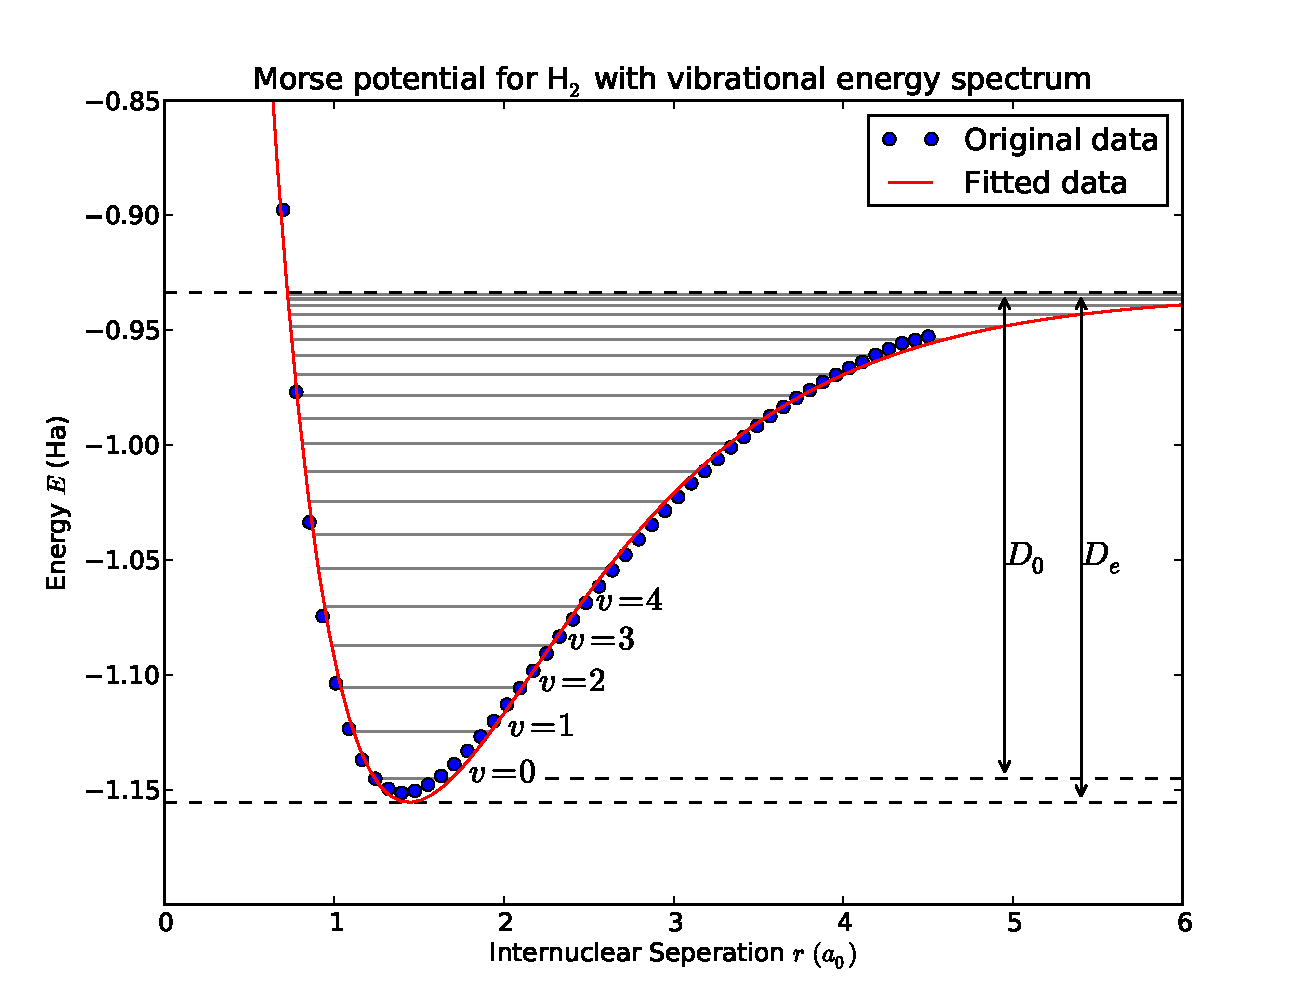
\includegraphics[width=\linewidth]{plot.pdf}
 \caption{The Morse potential (solid red) fitted to the data (blue dots). The fitting parameters are $r_e=1.441(6)$, the equilibrium bond distance with a corresponding energy of $E_0=-1.155(1)$, $D_e=0.221(2)$ the well depth and $a=0.97(1)$ the width of the well. The vibrational energy level spectrum is calculated for the potential and are plotted. The dissociation energy $D_e=-1.155(1)$ Ha is larger than the true energy required for dissociation $D_0=-1.145(1)$ Ha due to the zero point energy of the lowest ($v = 0$) vibrational level.}\label{fig:plot}
\end{figure}

Our goal was to solve the six-dimensional partial differential eigenvalue equation for the lowest eigenvalue $E_0$ at different internuclear distances $s$, and so trace out the potential $V(r)$. This potential should look much like the Morse potential; the depth and location of the minimum and the curvature of $V$ about this minimum are related to observable properties of the H$_2$ spectrum. The ground-state energy was calculated for 50 different values of $s$ in the range of $0.7\leq s \leq 4.5$, after which the Morse potential 

\begin{equation}
V(r) = D_e ( 1-e^{-a(r-r_e)} )^2 
\end{equation}

was fitted to the data. The results are depicted in figure \ref{fig:plot} and summarized in table \ref{H2}. The Schr\"odinger equation for the Morse oscillator is exactly solvable, giving the vibrational eigenvalues $\epsilon_v=\omega_0 (v+\frac12)-\frac{\omega_0^2}{4D_e}(v+\frac12)^2$ for $v=0,\;1,\;...\;,\;v_{max}$. The exponential parameter is given by $a=w_0\sqrt{\mu/2D_e}$, in which $\mu$ is the reduced mass \citep{morse1929diatomic}. Unlike the harmonic oscillator, the Morse potential has a finite number of bound vibrational levels with $v_{max} \approx 2D_e/\omega_0$, which in the case of H$_2$ is 20 and while in the harmonic oscillator potential the levels are evenly spaced by $\hbar \omega$, the Morse potential level spacing decreases as the energy approaches the dissociation energy. The vibrational energy spectrum is plotted in figure \ref{fig:plot}. The dissociation energy $D_e(=-1.155(1)$ Ha) is larger than the true energy required for dissociation $D_0(=-1.145(1)$ Ha) due to the zero point energy of the lowest ($v = 0$) vibrational level.\\

To find the dissociation energy of H$_2$, the energy of two isolated hydrogen atoms in its ground-state is subtracted from the depth of the well in the Morse potential $D_e$. In table \ref{D_e} our value is compared to experimental values and to values found with different methods in units of cm$^{-1}$, which it is an industry standard. It can readily be seen that our results are not as accurate as results reported in literature \citep{traynor1991quantum, szalewicz1986new, wolniewicz1983x} more than two decades ago. The reason for this is that they incorporated (non)-adiabatic, relativistic and radiative effects and also did not use the Born-Oppenheimer approximation. Furthermore, various trail wavefunctions were used which contained up to 20 parameters. Therefore we conclude that the present approach has provided good results for the small systems treated here. Especially, the error of the dissociation energy is within about 0.2\% of the exact energy if one utilizes a trial wavefunction that can generally be obtained by multiplying two Hartree-Fock single electron orbitals by a simple electron-electron Jastrow factor. So, it seems useful to apply the VMC method to the calculation of electronic energies and other physical quantities of larger systems.

\begin{table}
\caption{Results of H$_2$. We report the equilibrium internuclear distance $s$ and the corresponding ground-state energy found with the VMC and the fit parameter from the Morse potential. For the VMC 2000 walkers have been used and 100 000 displacements were attempted. The first 10 000 were removed from the data to ensure equilibrium. The expectation value for the energy $\left\langle E \right\rangle$ is given at the equilibrium distance. These values are compared to values found in experiments and other methods.}
\label{H2}
\centering
\begin{tabular}{llr}
\hline
$s$ ($a_0$) & $\left\langle E \right\rangle$ (Ha) & Method  \\ \hline
$1.405$ & $-1.151093(14)$ & Fit parameter \\
$1.411$ & $-1.15117(2)$   & VMC \\
$1.4011$ & $-1.17447593$ & Nonadiabatic \citep{wolniewicz1995nonadiabatic}
\end{tabular}
\end{table}

\begin{table}
\caption{Comparing the dissociation energy of H$_2$ ($D_0$)}\label{D_e}
\centering
\begin{tabular}{llr}
\hline
Method      & Reference                                   & Energy      \\ \hline
Exp.        & Herzberg \citep{herzberg1970dissociation}   & $36 117.3 \pm 1.0$ \\
Exp.        & Stwalley \citep{stwalley1970dissociation}   & $36 118.6 \pm 0.5$  \\
Nonadiabatic& Wolniewicz \citep{wolniewicz1983x}          & $36 118.1 \pm 0.5$ \\
Nonadiabatic& Kolos \citep{szalewicz1986new}              & $36 118.01 \pm 0.5$ \\
DQMC        & Traynor \citep{traynor1991quantum}          & $36 107 \pm 11$ \\
GFQMC       & Traynor \citep{traynor1991quantum}          & $36 118.6 \pm 2.0$ \\
VMC         & This work                                   & $36 219.8 \pm 70$  \\ \hline
\end{tabular}
\end{table}





%------------------------------------------------

% \section{Discussion}
% The present approach has provided good results for the small systems treated here. Especially, the error is within about 0.2\% of the exact energy when one utilizes a trial wavefunction that can generally be obtained by multiplying two Hartree-Fock single electron wavefunctions by a simple electron-electron Jastrow factor. So, it seems useful to apply the VMC method to the calculation of electronic energies and other physical quantities of larger systems.


%----------------------------------------------------------------------------------------
%	SECTION 4
%----------------------------------------------------------------------------------------


%----------------------------------------------------------------------------------------
%	BIBLIOGRAPHY
%----------------------------------------------------------------------------------------


\bibliography{mybib}{}
\bibliographystyle{plain}



%----------------------------------------------------------------------------------------

\section{Appendix}
\subsection{Derivation of local energies}
We will present the derivations for the atoms studied in this report
To evaluate the local energy we must work out $E_L$ in 
\begin{equation}
 \left\langle E \right\rangle = \frac{\int dR \Psi_T^2(R)E_L(R)}{\int dR \Psi_T^2(R)}
\end{equation}
in which $E_L$ is
\begin{equation}
 E_L(R)=\frac{\hat{H}\Psi_T(R)}{\Psi_T(R)}
\end{equation}
and
\begin{equation}
 \hat{H}=\sum_{i=1}^N \frac{p_i^2}{2m}+\frac12 \sum_{i\ne j=1}^N \frac{e^2}{\left| \mathbf{r}_i -\mathbf{r}_j \right|}+\sum_i V_{e-b}(\mathbf{r}_i)
\end{equation}

\subsubsection{Harmonic oscillator}
The Hamiltonian of the harmonic oscillator in dimensionless units is
\begin{equation}
 \hat{H}=-\frac12 \frac{d^2}{dx^2}+\frac12 x^2
\end{equation}

The exact ground state wavefunction is given by $e^{-x^2/2}$, we shall chose our trail variational wave function $\Psi_{T,\alpha}$ to be
\begin{equation}
 \Psi_{T}(x)=e^{-\alpha x^2}
\end{equation}

The local energy is \begin{equation}
 E_L(x)=\frac{\hat{H}\Psi_T(x)}{\Psi_T(x)}=\frac{1}{\Psi_T(x)} \left[ -\frac12 \frac{d^2}{dx^2}+\frac12 x^2 \right] \Psi_T(x)= -e^{\alpha x^2}\frac12 \frac{d^2}{dx^2}e^{-\alpha x^2}+\frac12 x^2
\end{equation}
in which $\frac{d^2}{dx^2}e^{\alpha x^2}=-2\alpha e^{-\alpha x^2}+4\alpha^2x^2e^{-\alpha x^2}$, so

\begin{equation}
 E_L(x)= -e^{\alpha x^2}\frac12 \frac{d^2}{dx^2}e^{-\alpha x^2}+\frac12 x^2=\alpha+ x^2 \left(\frac12 - 2\alpha^2 \right)
\end{equation}

\subsubsection{Hydrogen molecule H$_2$}

\begin{equation}
 \hat{H}=-\frac{\hbar}{2m}\left( \nabla_1^2 + \nabla_2^2 \right) - \left[ \frac{ke^2}{\left| \vec{r}_1 + \frac{s}{2} \hat{i} \right|} + \frac{ke^2}{\left| \vec{r}_1 - \frac{s}{2} \hat{i} \right|}  +\frac{ke^2}{\left| \vec{r}_2 + \frac{s}{2} \hat{i} \right|}  +\frac{ke^2}{\left| \vec{r}_2 - \frac{s}{2} \hat{i} \right|} \right] +\frac{ke^2}{\left| \vec{r}_1 + \vec{r}_2 \right|} 
\end{equation}
in which the first term is the kinetic energy of the two electrons. The part in the square brackets is the attraction between the nucleus and the electrons and the last term is the Coulomb interaction between the electrons. Setting the constants to unity, and setting $\vec{r}_{1L} = \vec{r}_1 + \frac{s}{2} \hat{i}$, $\vec{r}_{1R} = \vec{r}_1 - \frac{s}{2} \hat{i}$, $\vec{r}_{2L} = \vec{r}_2 + \frac{s}{2} \hat{i}$, $\vec{r}_{1R} = \vec{r}_2 - \frac{s}{2} \hat{i}$ and $\vec{r}_{12} = \vec{r}_1 -\vec{r}_2$ we obtain
\begin{equation}
\hat{H}=-\frac{1}{2}\left( \nabla_1^2 + \nabla_2^2 \right) - \left[ \frac{1}{|\vec{r}_{1L}|} +\frac{1}{|\vec{r}_{1R}|}+\frac{1}{|\vec{r}_{2L}|}+\frac{1}{|\vec{r}_{2R}|} \right] +\frac{1}{\left| \vec{r}_{12} \right|} 
\end{equation}
In the light of the solvability of this Hamiltonian we split it up in two non-interacting Hamiltonians and a interaction term.
\begin{equation}
 \hat{H}=\hat{H}_1 + \hat{H}_2 + \hat{H}_{ee}
\end{equation}

in which $\hat{H}_1=-\frac{1}{2}\nabla_1^2 - \frac{1}{|\vec{r}_{1L}|} -\frac{1}{|\vec{r}_{1R}|}$, $\hat{H}_2=-\frac{1}{2}\nabla_2^2 - \frac{2}{|\vec{r}_{1L}|} -\frac{2}{|\vec{r}_{2R}|}$ and $\hat{H}_{ee}=\frac{1}{|\vec{r}_{12}|}$

We have chosen our trail variational wave function $\Psi_{T,\alpha}$ to be
\begin{equation}
 \Psi_{T}(\vec{r}_1,\vec{r}_2)=\phi(\vec{r}_1)\phi(\vec{r}_2)\psi(\vec{r}_1,\vec{r}_2)
\end{equation}
where $\psi(\vec{r}_1,\vec{r}_2)$ is the Jastrow function

\begin{equation}
\psi(\vec{r}_1,\vec{r}_2) = \psi_{12} = e^{\frac{\left| \vec{r}_{12}  \right|}{\alpha(1+\beta |\vec{r}_{12}|)} }
\end{equation}

and $\phi(\vec{r}_1)$ and $\phi(\vec{r}_2)$ are
\begin{equation}
 \phi(\vec{r}_1) = e^{-|\vec{r}_{1L}|/a} + e^{-|\vec{r}_{1R}|/a} =\phi_1= \phi_{1L} +\phi_{1R}
\end{equation}


\begin{equation}
 \phi(\vec{r}_2) = e^{-|\vec{r}_{2L}|/a} + e^{-|\vec{r}_{2R}|/a} =\phi_2 = \phi_{2L} +\phi_{2R}
\end{equation}

\begin{equation}
 E_L(R)=\frac{\hat{H}\Psi_T(R)}{\Psi_T(R)}=\frac{1}{\phi_1\phi_2\psi_{12}} \hat{H} \phi_1\phi_2\psi_{12}
\end{equation}
We let the Hamiltonians only work on correct terms, which results in
\begin{equation}
 \frac{1}{\phi_1\phi_2\psi_{12}}(\hat{H}_1 + \hat{H}_2 + \hat{H}_{ee})\phi_1\phi_2\psi_{12}=\frac{1}{\phi_1\psi_{12}}\hat{H}_1 \phi_1\psi_{12} + \frac{1}{\phi_2\psi_{12}}\hat{H}_2 \phi_2\psi_{12} + \frac{1}{|\vec{r}_{12}|}
\end{equation}

Now we first consider
\begin{equation}
 \frac{1}{\phi_1\psi_{12}}\hat{H}_1 \phi_1\psi_{12} = - \frac{1}{\phi_1\psi_{12}} \frac12 \nabla_1^2(\phi_1\psi_{12}) - \frac{1}{|\vec{r}_{1L}|} -\frac{1}{|\vec{r}_{1R}|}
\end{equation}
from which we first consider $\nabla_1^2(\phi_1\psi_{12})$, using the chain rule 

\begin{equation}
\label{master}
\nabla_1^2(\phi_1\psi_{12}) = \psi_{12}\nabla_1^2\phi_1 + 2 \nabla_1\phi_1 \cdot \nabla_1  \psi_{12} + \phi_1\nabla_1^2\psi_{12}
\end{equation}
where
\begin{equation}
\label{no1}
 \nabla_1\phi_1 =-\frac1a \left( e^{-|\vec{r}_{1L}|/a} + e^{-|\vec{r}_{1R}|/a} \right)=-\frac1a \left(  e^{-|\vec{r}_{1L}|/a}\hat{r}_{1L} +e^{-|\vec{r}_{1R}|/a}\hat{r}_{1R} \right)
\end{equation}
and \footnote{from now on we will omit the vector signs when it's not ambiguous}

\begin{equation}
\label{no2}
 \nabla_1^2\phi_1 =  \left[\frac{1}{a^2}-\frac{2}{a{r}_{1L}} \right] e^{-{r}_{1L}/a} + \left[\frac{1}{a^2}-\frac{2}{a{r}_{1R}} \right] e^{-{r}_{1R}/a} 
\end{equation}

Similarly we find

\begin{equation}
\label{no3}
 \nabla_1 \psi_{12}= \nabla_1 \left( e^{\frac{{r}_{12} }{\alpha(1+\beta {r}_{12})} } \right) = \frac{e^{\frac{r_{12}}{\alpha (\beta r_{12}+1)}}}{\alpha (\beta r_{12}+1)^2}\hat{r}_{12}=\frac{\psi_{12}}{\alpha (\beta r_{12}+1)^2}\hat{r}_{12}
\end{equation}

and 

\begin{equation}
\label{no4}
 \nabla_1^2 \psi_{12}=e^{\frac{r_{12} }{\alpha(1+\beta r_{12} ) }} \frac{2\alpha \beta r_{12} + 2\alpha+r_{12}}{r_{12}\alpha^2(\beta r_{12}+1)^4} =  \frac{(1+2\alpha \beta) r_{12} + 2\alpha}{r_{12}\alpha^2(\beta r_{12}+1)^4} \psi_{12}
\end{equation}

Now substituting equations \ref{no1}, \ref{no2}, \ref{no3} and \ref{no4} into \ref{master}.
\begin{multline}
 \nabla_1^2(\phi_1\psi_{12}) =\psi_{12} \left( \left[\frac{1}{a^2}-\frac{2}{a{r}_{1L}} \right] e^{-{r}_{1L}/a} + \left[\frac{1}{a^2}-\frac{2}{a{r}_{1R}} \right] e^{-{r}_{1R}/a}  \right) +\\ \frac2a \left(  e^{-{r}_{1L}/a}\hat{r}_{1L} +e^{-{r}_{1R}/a}\hat{r}_{1R} \right)\frac{\psi_{12}}{\alpha (\beta r_{12}+1)^2}\hat{r}_{12} \\ +\left( e^{-|\vec{r}_{1L}|/a} + e^{-|\vec{r}_{1R}|/a} \right) \left(   \frac{(1+2\alpha \beta) r_{12} + 2\alpha}{r_{12}\alpha^2(\beta r_{12}+1)^4} \psi_{12} \right)
\end{multline}
shuffle to get

\begin{multline}
 \frac{\nabla_1^2(\phi_1\psi_{12})}{\phi_1 \psi_{12}} =\frac{1}{\phi_1} \left( \left[\frac{1}{a^2}-\frac{2}{ar_{1L}} \right] e^{-r_{1L}/a} + \left[\frac{1}{a^2} - \frac{2}{ar_{1R}} \right] e^{-{r}_{1R}/a}  \right)   
+ \\ \frac{1}{\phi_1 } \left(  e^{-{r}_{1L}/a}\hat{r}_{1L} +e^{-{r}_{1R}/a}\hat{r}_{1R} \right) \cdot \frac{2\hat{r}_{12}}{\alpha a(\beta r_{12}+1)^2}+    \frac{(1+2\alpha \beta) r_{12} 
+ 2\alpha}{r_{12}\alpha^2(\beta r_{12}+1)^4} 
\end{multline}
replace the exponents for the corresponding $\phi$ to obtain

\begin{multline}
\frac{\nabla_1^2(\phi_1\psi_{12})}{\phi_1 \psi_{12}} 
 = \left( \left[\frac{1}{a^2}-\frac{2}{ar_{1L}} \right] \frac{\phi_{1L}}{\phi_1} + \left[\frac{1}{a^2} - \frac{2}{ar_{1R}} \right] \frac{\phi_{1R}}{\phi_1}   \right)   
 + \\ \left(  \frac{\phi_{1L}}{\phi_1}\hat{r}_{1L} +\frac{\phi_{1R}}{\phi_1}\hat{r}_{1R} \right) \cdot \frac{2\hat{r}_{12}}{\alpha a(\beta r_{12}+1)^2}+    \frac{(1+2\alpha \beta) r_{12} 
 + 2\alpha}{r_{12}\alpha^2(\beta r_{12}+1)^4} 
\end{multline}

in which 

\begin{multline}
   \left[\frac{1}{a^2}-\frac{2}{a{r}_{1L}} \right] \frac{\phi_{1L}}{\phi_1} + \left[\frac{1}{a^2} - \frac{2}{a{r}_{1R}} \right] \frac{\phi_{1R}}{\phi_1}   \\ = \frac{1}{a^2} \left[ \frac{\phi_{1L}}{\phi_1} + \frac{\phi_{1R}}{\phi_1} \right]-\frac{2}{a\phi_1}\left[ \frac{\phi_{1L}}{r_{1L}}+\frac{\phi_{1R}}{r_{1R}} \right] \\ = \frac{1}{a^2} -\frac{2}{a\phi_1}\left[ \frac{\phi_{1L}}{r_{1L}}+\frac{\phi_{1R}}{r_{1R}} \right]
\end{multline}

Now adding the equations for the second electron, which are the same \footnote{up to one minus sign} because of the symmetry of the problem, multiplying with 1/2 and adding the Coulomb interaction terms to get

\begin{multline}
 E_L = -\frac{1}{a^2} +\frac{1}{a\phi_1}\left[ \frac{\phi_{1L}}{r_{1L}}+\frac{\phi_{1R}}{r_{1R}} \right] + \frac{1}{a\phi_2} \left[ \frac{\phi_{2L}}{r_{2L}}+\frac{\phi_{2R}}{r_{2R}}\right]
 + \\ \left(  \frac{\phi_{1L}}{\phi_1}\hat{r}_{1L} +\frac{\phi_{1R}}{\phi_1}\hat{r}_{1R}   -   \frac{\phi_{2L}}{\phi_2}\hat{r}_{2L} -\frac{\phi_{2R}}{\phi_2}\hat{r}_{2R}     \right)  \cdot \frac{\hat{r}_{12}}{\alpha a(\beta r_{12}+1)^2} \\
  -   \frac{(1+2\alpha \beta) r_{12} + 2\alpha}{r_{12}\alpha^2(\beta r_{12}+1)^4} 
  - \left[ \frac{1}{|\vec{r}_{1L}|} +\frac{1}{|\vec{r}_{1R}|}+\frac{1}{|\vec{r}_{2L}|}+\frac{1}{|\vec{r}_{2R}|} \right] +\frac{1}{\left| \vec{r}_{12} \right|} 
\end{multline}
with $\alpha=2$


 \begin{multline}
 E_L = -\frac{1}{a^2} + \frac{1}{a\phi_1}\left[ \frac{\phi_{1L}}{r_{1L}}+\frac{\phi_{1R}}{r_{1R}} \right] + \frac{1}{a\phi_2} \left[ \frac{\phi_{2L}}{r_{2L}}+\frac{\phi_{2R}}{r_{2R}}\right]
 + \\ \left(  \frac{\phi_{1L}\hat{r}_{1L}+\phi_{1R}\hat{r}_{1R}}{\phi_1}   -    \frac{\phi_{2L}\hat{r}_{2L}+\phi_{2R}\hat{r}_{2R}}{\phi_2}     \right) \cdot \frac{\hat{r}_{12}}{2 a(\beta r_{12}+1)^2} \\
  -   \frac{(1+4 \beta) r_{12} + 4}{4r_{12}(\beta r_{12}+1)^4} 
  - \left[ \frac{1}{|\vec{r}_{1L}|} +\frac{1}{|\vec{r}_{1R}|}+\frac{1}{|\vec{r}_{2L}|}+\frac{1}{|\vec{r}_{2R}|} \right] +\frac{1}{\left| \vec{r}_{12} \right|} 
\end{multline}

\subsection{Coulomb cusp condition}
When two Coulomb particles get close, the potential has  $1/r$ singularity. We want modify the wave function in such a way to cancel this singularity. Let us consider the case of an electron close to a nucleus. There are four cases to consider, but they will all lead to the same condition. We will only consider one case, that of the first electron approaching the left proton, which translates to the limits $r_{1L} \rightarrow 0$ and $r_{1R} \rightarrow s$. In this limit the $1/r_{1L}$ term blows up, but we can fix this by choosing the right variational parameter such that
\begin{equation}
 \hat{H}\phi_1=(-\frac12\nabla_1^2-1/r_{1L})\phi_1=0
\end{equation}
which is 

\begin{equation}
\label{cus}
\frac{1}{r_{1L}}= - \frac{1}{\phi_1} \frac12 \nabla_1^2 \phi_1 = -\frac{1}{\phi_1} \left( \frac{\phi_{1L}}{r_{1L}} + \frac{\phi_{1R}}{r_{1R}}  \right) + \frac{1}{a^2}
\end{equation}

Keeping only the singular term and writing the exponential functions for the $\phi$'s, we get

\begin{equation}
 \frac{1}{\phi_1} \frac{\phi_{1L}}{r_{1L}}= \frac{e^{-r_{1L}/a}}{e^{-r_{1L}/a}+e^{-r_{1R}/a}}\frac{1}{r_{1L}}
\end{equation}

Taking the limit $r_{1L} \rightarrow 0$ and comparing to equation (\ref{cus}) we find the condition we need to remove the singularity

\begin{equation}
 a(1+e^{-s/a})=1
\end{equation}

When taking the limit $r_{12} \rightarrow 0$, we find that the singularity is removed when we choose $\alpha=2$.

\section{The use of my program}
The program for H$_2$ can be found in \emph{VMC H2/vmc\_h2.f90}. One can adjust the parameters in a separate file \emph{vmc.params}. The results are written to separate files which are analysed with a Python script \emph{H2 Morse Potential.ipynb}, see the notebook on http://tinyurl.com/H2-iccp. All programs in the main folder will minimize the energy, but the programs in the folder \emph{Sequential} loop trough different values.\\

I have also completely written the VMC simulations for H, He and the harmonic oscillator in Python. The notebook can be found on http://tinyurl.com/iccp-vmc


\end{document}